%& --translate-file=cp1250pl
%bez powyzszej linijki nie dzialaja polskie znaki (musi ona byc w pierwszej linii dokumentu
%%&platex --translate-file=il2-pl % przeyestowac z tym
\documentclass[a4paper,12pt]{article}
\usepackage[polish]{babel}
\usepackage[T1]{fontenc}
\usepackage[dvips]{graphicx}

\usepackage[urlcolor=blue, colorlinks=true, bookmarks=true, bookmarksnumbered=true]{hyperref}
%\usepackage{intendfirst}
\usepackage{times}
\usepackage{epsfig}
\usepackage{color}

%ustawienie wielkosci akapitu
%\setlength{\parindent}{0mm}
%%odst�p mi�dzy akapitami
%\setlength{\parskip}{2mm}

%ustawienia rozmiaru tekstu
    \textwidth 16cm
    \textheight 24cm 
    \topmargin -15mm
    \evensidemargin-3mm
    \oddsidemargin -3mm

\begin{document}

%reszta
\section{Wprowadzenie}

Salomon to system do wydobywania wiedzy z danych zgodnie z metodologi� \emph{Knowlege Mining}.
Odkrywanie wiedzy to proces iteracyjny, podzielony na etapy. W ka�dym tym etapie wiedza jest poddawana
obr�bce. Etapy te mog� tworzy� cykle. Na ka�dym takim etapie proces odkrywania mo�e by� ukierunkowany zgodnie
z wymaganiami u�ytkownika. Ka�dy etap tworzy odr�bn� ca�o��. 

W Salomonie reprezentacj� etapu jest \emph{zadanie} (Task). Ka�de zadanie mo�e posiada� kilka nast�pnik�w i kilka
poprzednik�w. Ujmuj�c rzecz pro�ciej, zadania mog� by� zorganizowane w postaci grafu. 

Zadanie zdefiniowane jest jako tr�jka:
\begin{itemize}
	\item algorytm(dostarczany w postaci wtyczki, czyli \emph{pluginu}))
	\item dane steruj�ce algorytmem
	\item dane wej�ciowe, z kt�rych algorytm b�dzie wydobywa� wiedz�
\end{itemize}

Zadanie nie musi si� ogranicza� do danych, kt�re otrzyma�o z poprzedniego zadania. Ka�de zadanie ma
dost�p do ca�ej aktualnie zgromadzonej wiedzy i do wszystkich danych.

Na wej�ciu lub wyj�ciu ka�dego zadania mog� pojawi� si� dane (w przypadku algorytm�w, kt�re
dokonuj� selekcji/segregacji danych), wiedza lub obie te rzeczy naraz.

\begin{itemize}
	\item dane \begin{math}\Rightarrow \end{math} dane - najcz�ciej taki przypadek zdarza si� kiedy chcemy stworzy�
	zbiory treningowe lub zbiory testuj�ce
	\item dane \begin{math}\Rightarrow \end{math} wiedza - typowy przyk�ad wyszukiwania wiedzy: dostajemy dane, uzyskujemy wiedz�
	\item wiedza+dane \begin{math}\Rightarrow \end{math} dane - przypadek taki zachodzi kiedy chcemy wykorzysta� zgromadzon� wiedz� na dostarczonych danych
	\item wiedza \begin{math}\Rightarrow \end{math} wiedza
\end{itemize}

Celem tego projektu jest stworzenie przyjaznego �rodowiska do tworzenia, kontrolowania i efektywnego wykonywania zada� oraz przechowywania zgromadzonej wiedzy.

Salomon sk�ada si� z dw�ch zasadniczych cz�ci - pierwsz� z nich
stanowi platforma. Tworz� j�:
\begin{itemize}
	\item silnik, kt�rego zadaniem jest zarz�dzanie i~uruchamianie
zada�
	\item magazyn s�u��cy do przechowywania wiedzy
\end{itemize}

Druga cz�� to zbi�r wtyczek, dostarczaj�cych logik� potrzebn� do skonfigurowania, wykonania i~wy�wietlenia rezultat�w
zadania. System jest otwarty - oznacza to, �e jego funkcjonalno�� mo�e by� w �atwy spos�b rozszerzana poprzez dostarczenie nowych wtyczek.

\begin{figure}[htb]
	\centering
		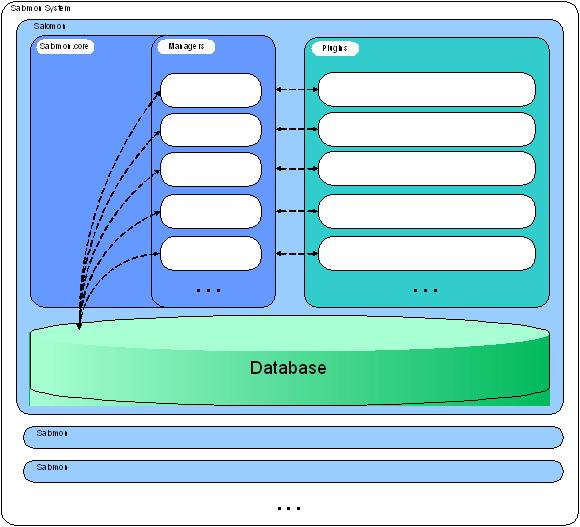
\includegraphics[width=0.90\textwidth]{img/uml/arch.jpg}
	\caption{Architektura systemu}
\end{figure}


\pagebreak
Podstawowe za�o�enia projektowe:
\begin{itemize}
    \item ca�a funkcjonalno�� w pluginach. J�dro systemu ma by� jak najmniejsze.
    Jego zadaniem jest stworzenie �rodowiska do realizacji logiki dostarczanej we wtyczkach
    \item otwarta~architektura. Wprowadzenie warstwy po�redniej pomi�dzy baz� danych~a wtyczkami.
    Jej zadaniem jest ukrycie sposobu organizacji danych przez
    wtyczkami. Otwarto��~architektury polega na mo�liwo�ci rozszerzenia tej warstwy
    \item niezale�no�� od platformy. System ma by� niezale�ny od platformy, mo�liwie �atwo przenaszalny.
    Poszczeg�lne cz�ci systemu mog� by� uruchamiane na r�nych
    platformach.
    \item mo�liwo�� wykorzystywania rezultat�w poprzednich zada� przez kolejne
    \item �atwa~adaptacja funkcjonalno�ci zawartej w \emph{Vinlenie}.
    Projekt powsta� jako platforma uruchomieniowa dla logiki zaimplementowanej w programie \emph{Vinlen},
    tworzonego pod kierownictwem prof. Ryszarda Michalskiego.    
\end{itemize}


Salomon ma na celu wyeliminowanie ogranicze� oryginalnego
\emph{Vinlena} poprzez wprowadzenie:

\begin{itemize}
    \item kolejkowania zada�
    \item rozproszenia
    \item r�wnoleg�o�ci
    \item rozszerzalno�ci (mechanizm wtyczek)
    \item przeno�no�ci (\emph{Java},\emph{Firebird})
\end{itemize}

\end{document}
